%!TEX program =pdflatex
\documentclass{beamer}
\usetheme{CambridgeUS}
%%define new comand
\def\argmin{\mathop{\rm arg~min}\limits}
\def\argmin{\mathop{\rm arg~min}\limits}
\newcommand{\bdelta}{\boldsymbol{\delta}}
\newcommand{\bbeta}{\boldsymbol{\beta}}
\newcommand{\bSigma}{\boldsymbol{\Sigma}}
\newcommand{\brho}{\displaystyle{\large{\boldsymbol{\rho}}}}
\newcommand{\bgamma}{\boldsymbol{\gamma}}
\newcommand{\bfeta}{\boldsymbol{\eta}}
\newcommand{\bPsi}{\boldsymbol{\Psi}}
\newcommand{\bmu}{\boldsymbol{\mu}}
\newcommand{\bvartheta}{\boldsymbol{\vartheta}}
\newcommand{\bzero}{\mathbf{0}}
\newcommand{\bone}{\mathbf{1}}
\newcommand{\bA}{\mathbf{A}}
\newcommand{\ba}{\mathbf{a}}
\newcommand{\bB}{\mathbf{B}}
\newcommand{\bb}{\mathbf{b}}
\newcommand{\bD}{\mathbf{D}}
\newcommand{\bU}{\mathbf{U}}
\newcommand{\bu}{\mathbf{u}}
\newcommand{\bV}{\mathbf{V}}
\newcommand{\bW}{\mathbf{W}}
\newcommand{\bw}{\mathbf{w}}
\newcommand{\bX}{\mathbf{X}}
\newcommand{\bx}{\mathbf{x}}
\newcommand{\bY}{\mathbf{Y}}
\newcommand{\by}{\mathbf{y}}
\newcommand{\bZ}{\mathbf{Z}}
\newcommand{\bz}{\mathbf{z}}
\newcommand{\suit}[1]{\left(#1\right)}
\newcommand{\abs}[1]{\left\vert#1\right\vert}
\newcommand{\set}[1]{\left\{#1\right\}}
\newcommand{\msuit}[1]{\left[ #1 \right]}
\author{Laurens de Haan and Chen Zhou }
\date{Dec, 07, 2020}
\title{Trends in Extreme Value Index}
\begin{document}
\begin{frame}
\titlepage
\begin{center}
    Published on Journal of the American Statistical Association(2020).

    \bigskip
    Presented by Liujun Chen

\end{center}
\end{frame}


\AtBeginSection[]
{
    \begin{frame}
        \frametitle{Table of Contents}
        \tableofcontents[currentsection]
    \end{frame}
}


\section{Introduction}

\begin{frame}
    \frametitle{Background}
\begin{itemize}
    \item Classic extreme value analysis assumes that the observations are i.i.d.
    \bigskip
    \item Recent studies aim at dealing with the case when observations are drawn from different distributions.
    \bigskip
    \item This paper considers a continuously changing extreme value index and try to estimate the functional extreme value index accurately.
\end{itemize}
\end{frame}

\begin{frame}
    \frametitle{Model Setting}
\begin{itemize}
    \item Consider a set of distributions $F_s(x)$ for $s\in [0,1]$ and independent random variables $X_i\sim F_{\frac{i}{n}}(x)$ for $i=1,\dots,n$.
    \medskip
    \item Here $F_s(x)$ is assumed to be continuous with respect to $s$ and $x$. And assume that $F_s \in D_{\gamma(s)}$.
    \medskip
    \item This article considers the case that the function $\gamma$ is positive and continuous on $[0,1]$.
    \medskip
    \item The goal is to estimate the function $\gamma$ and test the hypothesis that $\gamma=\gamma_0$ for some given function $\gamma_0$.
\end{itemize}

\end{frame}



\section{Methodology}

\begin{frame}
    \frametitle{Methodology}
\begin{itemize}
    \item The idea for estimating $\gamma(s)$ locally is similar to the kernel density estimation.
    \medskip
    \item More specifically, use only observations $X_i$ in the $h$-neighborhood of $s$, that is 
    $$
i\in I_n(s)=\set{\abs{\frac{i}{n}-s}\le h},
    $$
    where $h:=h(n)$ is the bandwidth such that as $n\to \infty$, $h \to \infty$ and $nh\to \infty$.
    \medskip
\item Correspondingly, there will be $[2nh]$ observations for $s\in [h,1-h]$.
\end{itemize}
\end{frame}

\begin{frame}
    \frametitle{Local estimator}
\begin{itemize}
    \item To apply any known estimators for extreme value index, such as Hill estimator, choose am intermediate sequence $k=k(n)$ such that $k\to \infty, k/n \to 0$ as $n \to \infty$.
    \item Then one can use the top $[2kh]$ order statistics among the $[2nh]$ local observations in the $h$-neighborhood of $s$ to estimate $\gamma(s)$.
    \item The local Hill estimator for $\gamma(s)$ is defined as follows. Rank the $[2nh]$ observations $X_i$ with $i \in I_n(s)$ as $X_{1,[2nh]}^{(s)}\le \cdots \le X_{[2nh],[2nh]}^{(s)}$. Then
    $$
    \hat{\gamma}_{H}(s):=\frac{1}{[2 k h]} \sum_{i \in I_{n}(s)}\left(\log X_{i}-\log X_{[2 n h]-[2 k h],[2 n h]}\right)^{+}.
    $$
\end{itemize}
\end{frame}







\begin{frame} 
    \frametitle{Second order condition}
To obtain the asymptotic theory, the following conditions are required.
   
\bigskip

First, the second order condition is assumed. Suppose there exists a continuous negative function $\rho(s)$ on $[0,1]$ and a set of auxiliary function $A_s(t)$ that are continuous with respect to $s$, such that
\begin{equation}\tag{3}
    \lim _{t \rightarrow \infty} \frac{\frac{U_{s}(t x)}{U_{s}(t)}-x^{\gamma(s)}}{A_{s}(t)}=x^{\gamma(s)} \frac{x^{\rho(s)}-1}{\rho(s)},   
\end{equation}


holds for $x>1/2$ and uniformly for all $s\in [0,1]$. 
\end{frame}


\begin{frame}
    \frametitle{Conditions for $k$ and $h$}
Choose the intermediate sequence $k$ and the bandwidth $h$ as follows:
\begin{itemize}
    \item \begin{equation}\tag{4}
        h=h_n\to 0, k=k_n \to \infty, k_n/n \to 0, \dfrac{k_nh_n}{|\log h_n|}\to \infty,   
    \end{equation}
 


\item \begin{equation}\tag{5}
    \Delta_{1,n}:=\sqrt{k_n}\sup_{0\le s\le 1}|A_s(\dfrac{n}{k_n})|\to 0 
\end{equation}

  

\item \begin{equation}\tag{6}
    \Delta_{2, n}:=\sqrt{k_{n}} \log k_{n} \sup _{\left|s_{1}-s_{2}\right| \leq 2 h_{n}}\left|\gamma\left(s_{1}\right)-\gamma\left(s_{2}\right)\right| \rightarrow 0.  
\end{equation}



\item \begin{equation}\tag{7}
    \Delta_{3, n}:=\sup _{\left|s_{1}-s_{2}\right| \leq h_{n}}\left|\frac{\frac{U_{s_{1}}\left(\frac{n}{k_{n}}\right)}{U_{s_{2}}\left(\frac{n}{k_{n}}\right)}-1}{A_{s_{2}}\left(\frac{n}{k_{n}}\right)}\right| \rightarrow 0 
\end{equation}
\end{itemize}
    

\end{frame}


\begin{frame}
    \frametitle{Theorem 2.1: Asymptotical normality of the local estimator}

    \begin{theorem}[2.1]
        Let $X_1,X_2,\dots, X_n$ be independent random variables with distributions $X_i \sim F_{\frac{i}{n}}(x)$, where $F_s(x)$ is a set of distribution functions depends on $s\in [0,1]$. Assume that $F_s(x)$ is continuous with respect to $x$ and $s$ and $F_s \in D_{\gamma(s)}$ where $\gamma(s)$ is a positive continuous function on [0,1]. Assume conditions (3)-(7). Then as $n \to \infty$, we have that for all $s\in (0,1)$, 
$$
\sqrt{2kh}(\hat{\gamma}_H(s)-\gamma(s))\stackrel{d}{\to}N(0,\gamma^2(s)).
$$    
    \end{theorem}
\end{frame}

\begin{frame}
    \frametitle{Main difficulties of the proofs}

    

\end{frame}




\begin{frame}
    \frametitle{Global Estimator}
Next, consider testing the hypothesis that $\gamma(s)=\gamma_0(s)$ for all $s\in [0,1]$.

\bigskip

\begin{itemize}
    \item Although Although we are able to estimate the function $\gamma$ locally, since the local estimators use only local observations, their asymptotic limits are obviously independent. {\color{red} What does this mean?}
    \item In addition, the local estimator converges with a slow speed of convergence $1/\sqrt{2kh}$.
    \item  To achieve the stated goal, we consider the estimation $\Gamma(s)=\int_{0}^{s}\gamma(u)du$ and test the equivalent hypothesis that $\Gamma=\Gamma_0$.
\end{itemize}
\end{frame}

\begin{frame}
    \frametitle{Global Estimator}

    \begin{itemize}
        \item      Consider a discretized version of $\hat{\gamma}_H(s): \hat{\gamma}_H\suit{(2[\dfrac{s}{2h}]+1)h}$.
        \smallskip
        \item      Define the estimator of $\Gamma(s)$ as the integral of the discretized version as follows: for all $0\le s\le 1$,
        $$
        \hat{\Gamma}_{H}(s)=\int_{0}^{s} \hat{\gamma}_{H}\left(\left(2\left[\frac{u}{2 h}\right]+1\right) h\right) d u.
        $$
        \smallskip
        \item Note that $\hat{\gamma}_H(s)$ is only defined for $s\le 1-h$.
        \smallskip
        \item For $u>1-h$, we may have $(2[\dfrac{s}{2h}]+1)h=(2[\dfrac{1}{2h}]+1)h$. Then we extend the range of the estimator and define $\hat{\gamma}_H((2[\dfrac{s}{2h}]+1)h):=\hat{\gamma}_H((2[\dfrac{s}{2h}]-1)h)$
    \end{itemize}


\end{frame}


\begin{frame}
    \frametitle{Asymptotic Properties of the Global Estimator}

    \begin{theorem}[2.2]
        Assume the same conditions in Theorem 2.1. Then under a Skorokhod  construction, there exists a series of Brownian motions $W_n(s)$ such that as $n \to \infty$,
$$
\sup _{s \in[0,1]}\left|\sqrt{k}\left(\hat{\Gamma}_{H}(s)-\Gamma(s)\right)-\int_{0}^{s} \gamma(u) d W_{n}(u)\right| \stackrel{P}{\rightarrow} 0.
$$
    \end{theorem}
    

\end{frame}


\begin{frame}
    \frametitle{Sketch of the proofs}

    

\end{frame}

\begin{frame}
    \frametitle{Testing Trends in Extreme Value Indices}
The null hypothesis is $H_0: \Gamma(s)=\Gamma_0(s)$ for all $s$.

\bigskip

Clearly, one may construct the Kolmogrov-Smirnov(KS) type test with the testing statistic defined as 
$$
T:=\sup_{s\in [0,1]} \abs{\hat{\Gamma}_H(s)-\Gamma_0(s)}.
$$

Then by Theorem 2.2, under the null hypothesis $H_0$,
$$
\sqrt{k} T \stackrel{d}{\rightarrow} \sup _{s \in[0,1]}\left|\int_{0}^{s} \gamma(u) d W(u)\right|.
$$
\end{frame}

\begin{frame}
    \frametitle{Testing Trends in Extreme Value Indices}
    It is often of interest to test whether the extreme value index remains constant over time, that is, $H_0 :\gamma(s)=\gamma$ for all $s \in [0,1]$ without specifying $\gamma$. In this case, one may use $\hat{\Gamma}_H(1)$  as an estimator of the constant extreme value index $\gamma$ and define the testing statistic as
    $$
    \tilde{T}:=\sup _{s \in[0,1]}\left|\frac{\hat{\Gamma}_{H}(s)}{\hat{\Gamma}_{H}(1)}-s\right|.
    $$
    It is straightforward to show under $H_0$, as $n \to \infty$
    $$
    \sqrt{k} \tilde{T} \stackrel{d}{\rightarrow} \sup _{s \in[0,1]}|B(s)|,
    $$
    where $B(s)$ is a standard Brownian bridge defined on [0,1].
\end{frame}


\section{Simulation Study}

\begin{frame}
    \frametitle{Simulation Setting}
Run a simulation study to demonstrate the finite sample performance of the testing procedure using $\tilde{T}$.

\begin{itemize}
    \item $m=2000$ samples
    \item  $n=2000$ observations in each sample
    \item  $k=100,200$
    \item  $h=0.025,0.04$
\end{itemize}
  
    
    For each sample,  simulate the observations from the following data generating process
    $$
    X_i=Z_i^{1/\gamma(i/n)}, i=1,2,\dots,n,
    $$
    where $\{Z_i\}_{i=1}^n$ are iid observations from the standard Fr\'echet distribution.
\end{frame}

\begin{frame}
    \frametitle{Simulation Setting}
    For the function $\gamma(s)$ we consider 
    \begin{itemize}
        \item  either a linear trend as $\gamma(s)=1+bs$
        \item  or a trend following the sin function as $\gamma(s)=1+c\sin(2\pi s)$.
        \item 
        If $b=0$ or $c=0$, the two model resemble the iid case.
        \item     
        Consider four alternative cases $b=1, b=2, c=1/4$ and $c=1/2$.
    \end{itemize}
\end{frame}



\begin{frame}
    \frametitle{QQ plots for $b=0$}
\begin{center}
    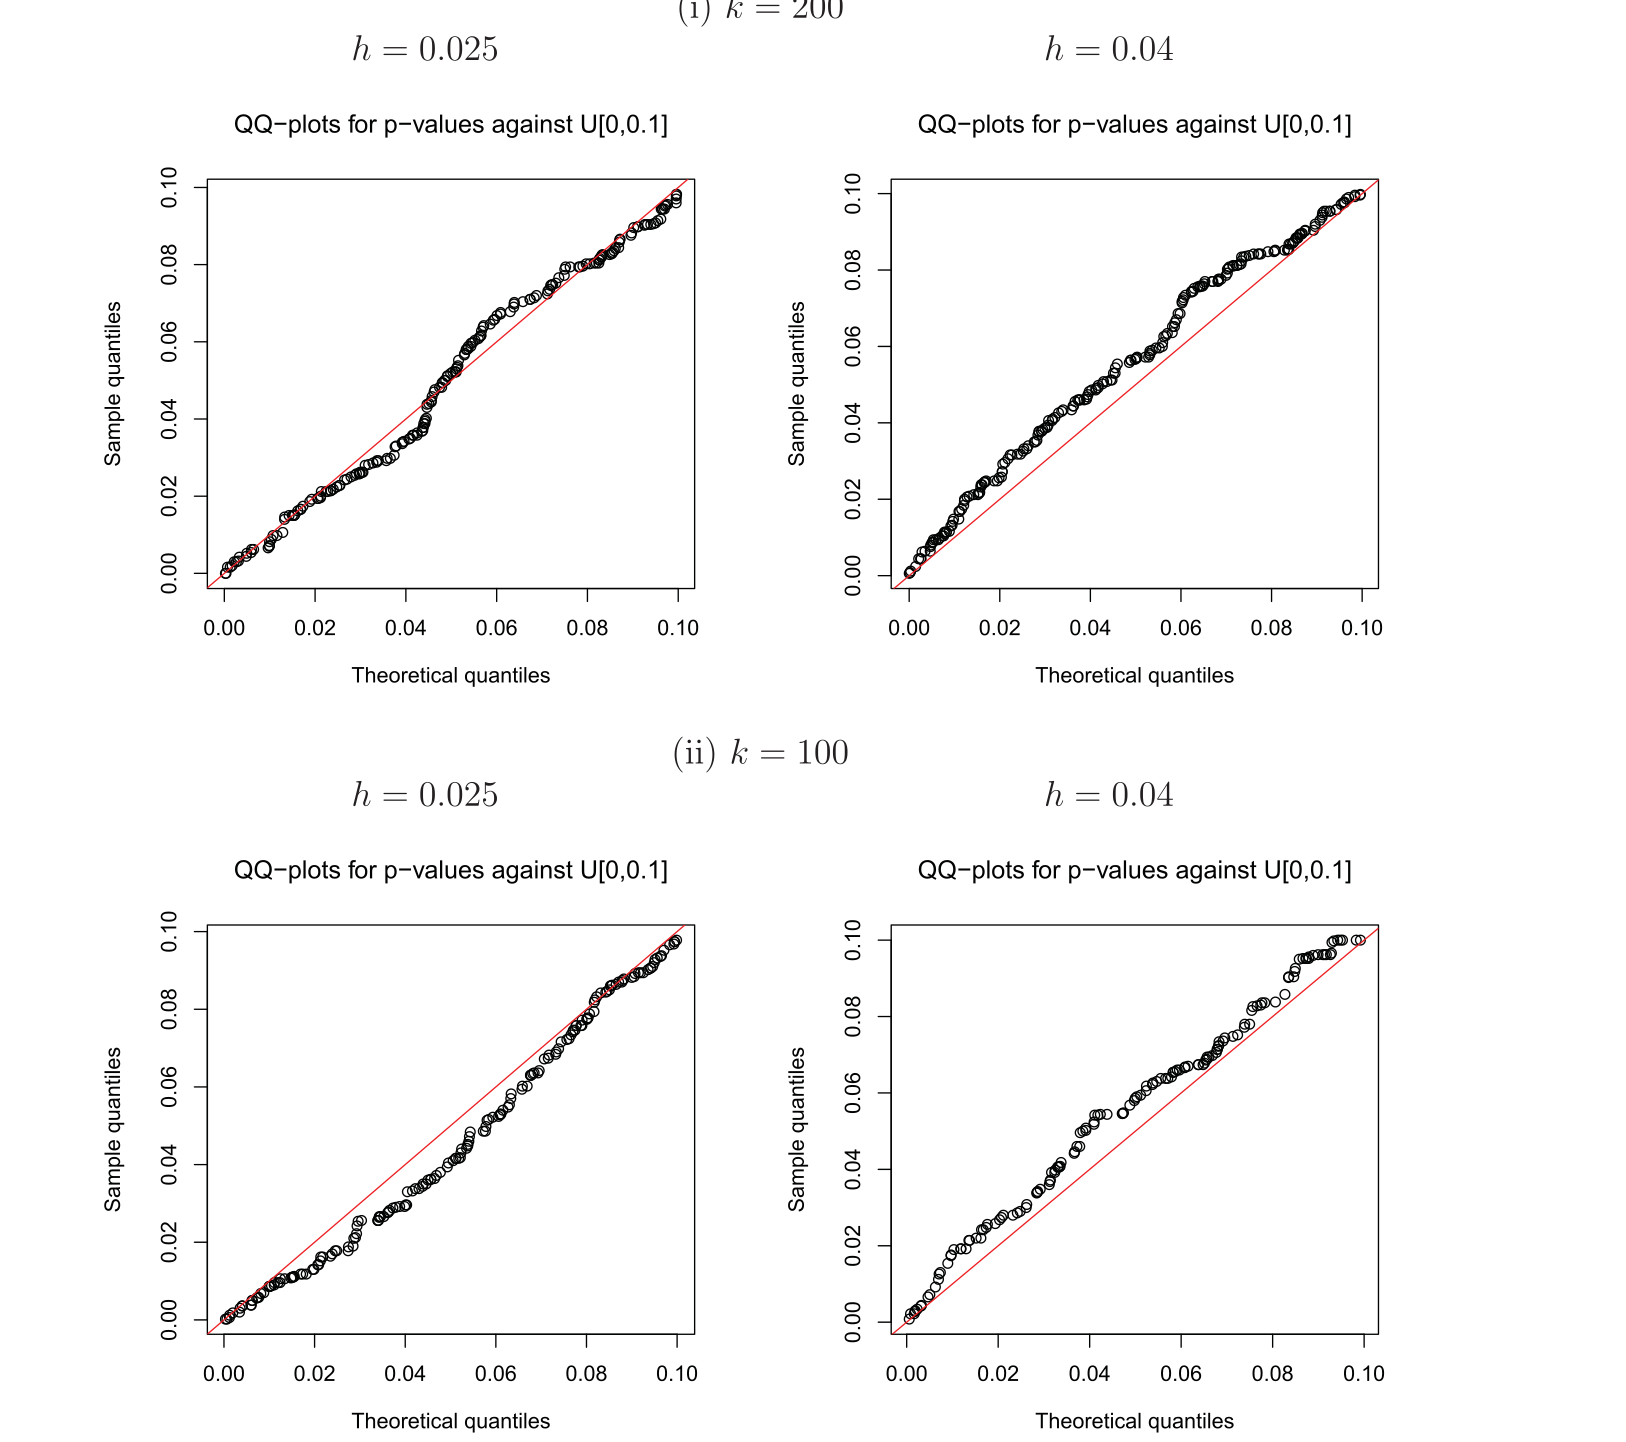
\includegraphics[width=0.7\textwidth]{QQ.png}
\end{center}
\end{frame}

\begin{frame}
    \frametitle{Rejection Rate}

    \begin{center}
        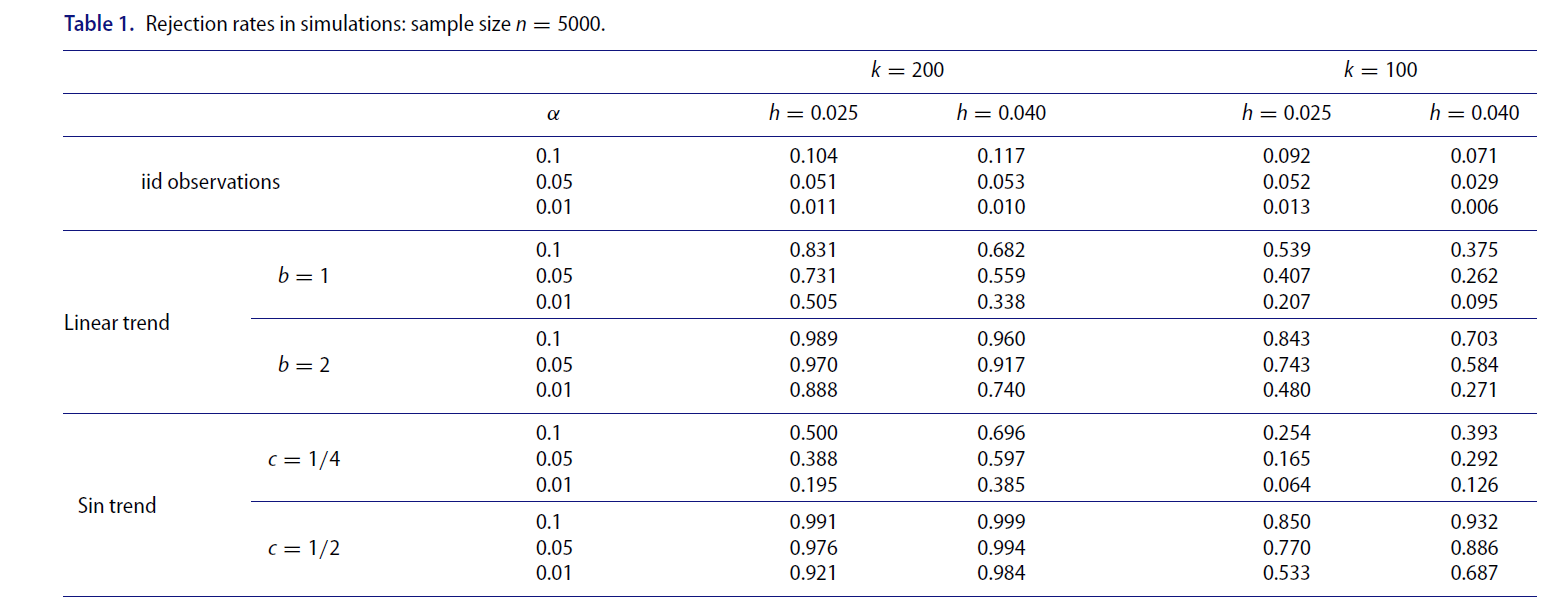
\includegraphics[width=1\textwidth]{image-20200429225741056}
    \end{center}

\end{frame}

\begin{frame}
    \frametitle{Estimated varying extreme value index: sin trends}
\begin{center}
    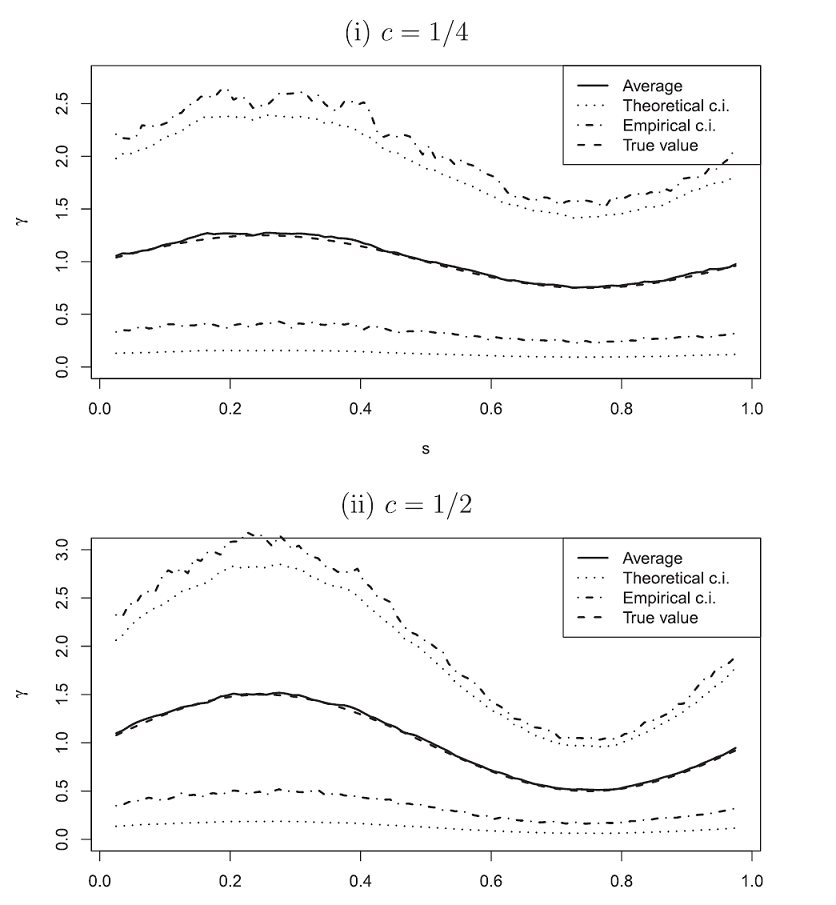
\includegraphics[width=0.58\textwidth]{image-20200429225848297}
\end{center}
    

\end{frame}
\section{Application}

\begin{frame}
    \frametitle{Preciptiattion at Saint-Martin-de-Londres}

\begin{itemize}
    \item A dataset consisting of the precipitation at Saint-Martin-de-Londres from 1976 to 2015, with 14,610 daily observations.
    \medskip
    \item Test the constancy of the extreme value indices over the entire period.
    \medskip
    \item Do not reject the null hypothesis under the 5% significance level (the dash line).
    \medskip
    \item Estimate the constant extreme value index by applying the Hill estimator to all observations, that is, estimating $\Gamma(1)$.
\end{itemize}
\end{frame}

\begin{frame}
    \frametitle{Testing the constancy of EVI:preciptation}
\begin{center}
    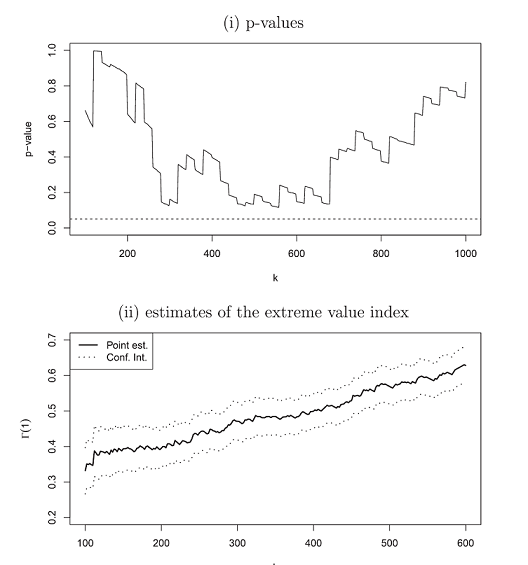
\includegraphics[width=0.59\textwidth]{image-20200429230720801}
\end{center}
    

\end{frame}


\begin{frame}
    \frametitle{Application 2: loss Return of S\&P 500}

   \begin{itemize}
       \item  S\&P 500 index 1988-2012(n=6302) \& 1963-2012(n=12586).
       \bigskip
       \item Daily loss returns are defined as $X_t=\log (P_t/P_{t+1})$
   \end{itemize} 
\end{frame}

\begin{frame}
    \frametitle{Testing the constancy of EVI: S\&P500}
\begin{center}
    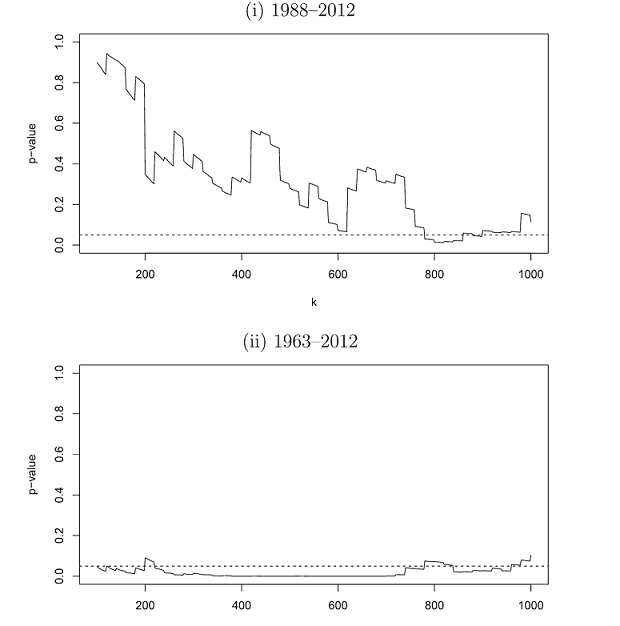
\includegraphics[width=0.6\textwidth]{image-20200429230846070}
\end{center}
    

\end{frame}

\begin{frame}
    \frametitle{Serial Dependence}
\begin{itemize}
    \item Financial data such as stock returns exhibits serial dependence. Correspondingly, the critial value of the proposed test should be higher.
    \bigskip
    \item By using the test based on assuming no serial dependence, we tent to over reject the null.
    \bigskip
    \item Given that the analysis using the data from 1988to 2012 did not reject the null, accounting for serial dependence may not alter the conclusion. However, the rejection resultbased on the data from 1963 to 2012 may suffer from the serialdependence issue. 
\end{itemize}
    

\end{frame}

\begin{frame}
    \frametitle{Testing the constancy of EVI: S\&P500}

    \begin{center}
        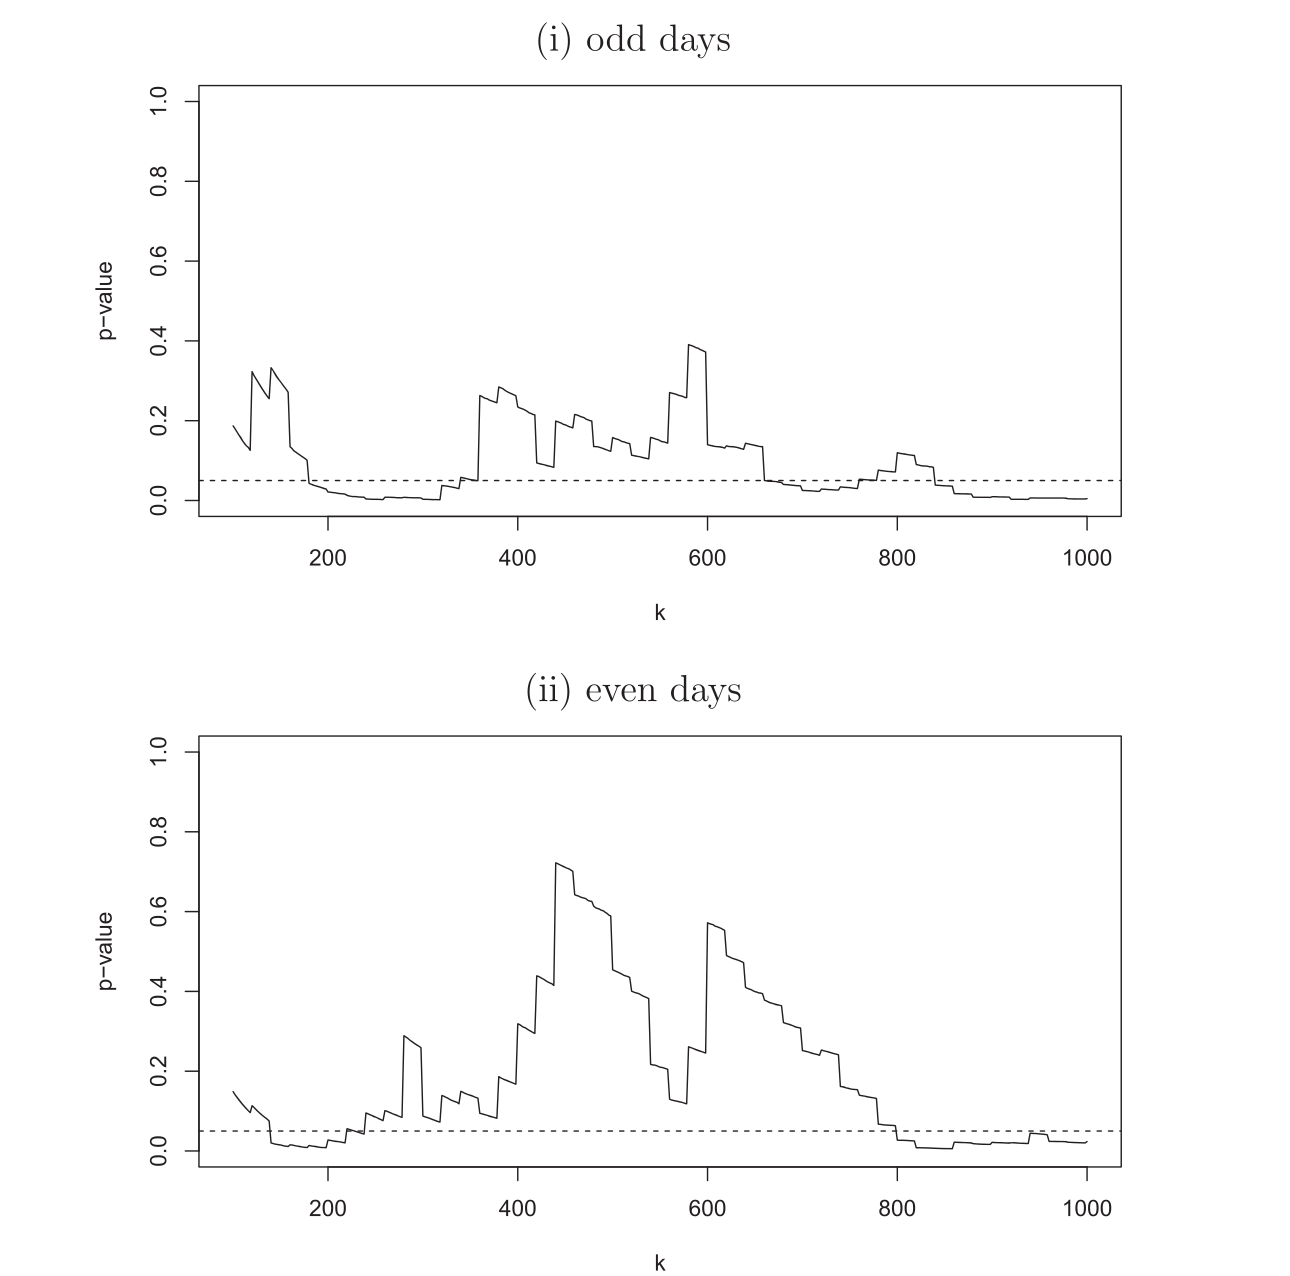
\includegraphics[width=0.65\textwidth]{Figure6}
    \end{center}

\end{frame}

\begin{frame}
    \frametitle{}
\begin{center}
    \LARGE Thanks!
\end{center}
    

\end{frame}
\end{document}